\subsubsection{Постановка задачи}
\label{sec:data_req}
Одной из ключевых задач исследования являлся сбор данных. Как отмечалось, корпус формировался с учётом
требований универсальности и перспективы дальнейшего использования в смежных исследованиях.

\textbf{Требования к данным.} В качестве основного источника качественных данных выбраны тексты.
В финансовом домене наиболее ёмкими и значимыми по влиянию на стоимость активов являются:

\begin{itemize}
    \item новостные статьи;
    \item посты в социальных сетях;
    \item официальные отчёты (годовые, квартальные, стратегические);
    \item пресс-релизы;
    \item аналитические обзоры и статьи;
    \item транскрипты интервью, конференций и веб-трансляций публичных компаний.
\end{itemize}

Предыдущие исследования подтвердили эффективность этих типов текстов. Так, FinBERTv3 \parencite{Yang2020FinBERT,Huang2023FinBERT}
обучался на официальных отчётах и аналитических статьях, а его вторая версия включала пресс-релизы \parencite{Liu2020FinBERT}.
Другие модели тонко настраивались под задачу анализ тональности на заголовках новостей и публикациях из социальных сетей
\parencite{Araci2019FinBERT}. Тем не менее в рамках нашего исследования целенаправленно обрабатываются полные тексты
без их фрагментации. Официальные отчёты часто превышают 8192 токена, которые способен обработать ModernBERT,
что затрудняет их интеграцию, тогда как слишком короткие форматы (посты в социальных сетях) не раскрывают
преимущества работы с длинным контекстом.

Кроме того, нет единого источника, агрегирующего все перечисленные типы текстов. Ввиду чего, обращая внимание
на ограниченность ресурсов, для первичной фокусировки были выбраны наиболее значимые виды:

\begin{itemize}
    \item новостные статьи;
    \item аналитические обзоры и статьи;
    \item пресс-релизы;
    \item транскрипты финансовых мероприятий.
\end{itemize}

В будущем планируется расширить корпус другими категориями контента.

Для обеспечения универсальности и удобства дальнейшего использования для каждого текста были собраны следующие следующие метаданные:

\begin{itemize}
    \item заголовок (например, «Covestro board enters formal talks on \$12 billion ADNOC approach»);
    \item источник (правообладатель), например, Reuters, Simply Wall St., PR Newswire, @ilyasut, Max Gottich;
    \item ресурс, на котором был опубликован текст (например, Twitter, Yahoo! Finance, Reddit, Seeking Alpha);
    \item дата и время публикации по UTC с точностью до секунды (например, 2024-09-01T01:48:13);
    \item тематические метки от автора (например, ["M\&A", "Cryptocurrency", "Tech"]);
    \item список тикеров, ассоциированных автором с текстом (например, ["9626.HK", "BILI"]).
\end{itemize}

В заключении был установлен оптимальный период для сбора данных. Нижняя и верхняя границы дат подбирались
исходя из предположения о том, что данный корпус в дальнейшем будет использоваться для обучения модели предсказания
стоимости, что обязывает синхронизировать первоначальные знания ModernBERT с теми, на которых он позднее будет
тонко настраиваться. По причине того, что в публикации ModernBERT не раскрываются данные на которых была обучена
модель, невозможно точно судить о том, за какой период были взяты данные \parencite{Warner2024ModernBERT}. Посему в нашем исследовании, ориентируясь
на дату публикации ModernBERT \parencite{Warner2024ModernBERT} и классического соотношения обучающей, валидационной и тестовой выборок как 75/15/10
был принят диапазон дат с 17.09.2023 по 18.03.2025, то есть 548 дней, из которых 374 рабочие по календарю США.

\textbf{Требования к источникам.} Источники данных должны быть открытыми, бесплатными, англоязычными и авторитетными,
поскольку широкий охват и оперативность публикаций напрямую влияют на реакцию рынков. В числе рассматриваемых
источников оказались:

\begin{itemize}
    \item Новостные издания: Bloomberg\footnote{URL: \url{https://www.bloomberg.com/}},
    The New York Times\footnote{URL: \url{https://www.nytimes.com/}},
    Reuters\footnote{URL: \url{https://www.reuters.com/}}, etc;
    \item Аналитические платформы: Seeking Alpha\footnote{URL: \url{https://seekingalpha.com/}},
    TradingView\footnote{URL: \url{https://tradingview.com/}};
    \item Официальные сайты: корпоративные и правительственные порталы.
\end{itemize}

При анализе более 50 корпоративных и более 100 правительственных ресурсов установлено,
что благодаря наличию RSS-лентам, пресс‑релизы централизованно агрегируются через PR Newswire\footnote{URL: \url{https://www.cision.com/}}
и GlobeNewswire\footnote{URL: \url{https://www.globenewswire.com/}}. Имеется и ряд других автоматических агрегаторов, например,
Business Wire\footnote{URL: \url{https://www.businesswire.com/}}),
ACCESS Newswire и других, однако эмпирически было выявлено, что среди подобных агрегаторов
доминируют PR Newswire и GlobeNewswire. Тем не менее, данные агрегаторы не дают разнообразия жанров.

Из новостных изданий по скорости реакции и охвату рынков оптимальной признана служба Reuters.
Также было изучено несколько более узких, но качественных источников (например, The Information\footnote{URL: \url{https://www.theinformation.com/}},
Epoch AI\footnote{URL: \url{https://epoch.ai/}}), однако они содержат слишком узкоспециализированную информацию, в то время как более
традиционные источники по типу Bloomberg, Wall Street Journal\footnote{URL: \url{https://www.wsj.com/}},
The Economist\footnote{URL: \url{https://www.economist.com/}} и другие покрывают более обширную часть рынков, однако технически ограничены.

Среди аналитических платформ Seeking Alpha уступает из‑за большого объёма платного контента,
а TradingView не обеспечивает доступ к историческим публикациям.

Таким образом, основными первичными источниками корпуса стали PR Newswire и Reuters. Однако, чтобы снизить риск
систематической предвзятости и обеспечить дополнительный охват, принято решение обогатить корпус другими
издательствами, но в силу их разрозненности, отсутствия API, а также зачастую и полной информации о статье
(включая время публикации с точностью о секунды), агрегировать и синхронизировать данные не представляется возможным.
Так, дополнительно были рассмотрены агрегаторы Google Finance\footnote{URL: \url{https://www.google.com/finance/}},
Yahoo! Finance\footnote{URL: \url{https://finance.yahoo.com/}} и FinURLs\footnote{URL: \url{https://finurls.com/}}.

В итоге предпочтение отдано Yahoo! Finance благодаря унифицированной схеме сайта и широкому отражению разнообразных
источников, тогда как FinURLs использует переадресацию на сайты источников, каждый из которых имеет свою собственную
схему сайта. С другой стороны, Google Finance больше похож на Yahoo! Finance, однако не предоставляет возможности
для сбора исторических данных.


\subsubsection{Сбор данных}
\label{sec:data_collecting}

Предваряя сбор данных, был проведен поиск и анализ существующих открытых решений для сбора данных
с Yahoo! Finance. В ходе анализа выявлено пять наиболее подходящих инструментов. При этом два --- 'yahooquery'
и 'yahoo-stock-api' --- не поддерживают извлечение статей, ещё два --- 'yahoo\_fin' и 'fin-news' --- оказались
заброшенными и не работают должным образом, а 'yfinance' предоставляют доступ исключительно к последним двадцати
новостным материалам в реальном времени. В связи с этим была разработана собственная программа‑парсер на языке Python.
Архитектура парсера состоит из двух ключевых этапов.

\begin{enumerate}
    \item Сбор ссылок. Рекурсивный обход официальной карты сайта позволяет собрать ссылки на статьи за заданный период.
    Каждая «страница дня» содержит 50 ссылок на новости и указатель на следующую страницу, причём доступ к странице $n$
    возможен только через страницу $n-1$, что являлось узким местом процесса парсинга, имплементируя связанный список
    с высокой сетевой задержкой.
    \item Извлечение содержимого. По собранным URL-адресам производится парсинг текстов статей. Важно отметить,
    что, как и для обучения классической модели BERT, таблицы и изображения не обрабатывались \parencite{devlin2019BERT}.
\end{enumerate}

В ходе парсинга было выявлено множество ограничений, которые затем были учтены при разработке архитектуры программы-парсера:

\begin{itemize}
    \item IP-блокировки и cookies. Инфраструктура Yahoo! Finance ограничена 14 параллельными запросами с одного IP
    с интервалом не менее 4 секунд; при нарушении интервалов ответы содержат коды 404, 429 или 200 с пустым телом. Тем не менее,
    как оказалось, даже с выполнением всех инфраструктурных требований, данная проблема все равно может возникать. Для обхода
    блокировок использовался пул из 50 прокси-серверов, а неудачные запросы автоматически обрабатывались в дополнительной итерации.
    \item Региональные ограничения. Из разных стран одни и те же ссылки мгуть быть недоступны или работать некорректно.
    \item Технические неполадки. Встречались ссылки с переадресацией на внешние источники, битые и платные ссылки,
    которые игнорировались в ходе сбора корпуса.
\end{itemize}

Для ускорения обработки больших объёмов данных была использована библиотека реализованная на C --- 'selectolax' ---
которая в 30 раз быстрее 'BeautifulSoup' и в 5 раз — 'lxml'.

В результате на первом этапе было собрано 1 362 103 ссылки, из которых 1 360 761 принадлежали домену Yahoo! Finance.
Успешно спаршено 1 304 717 статей благодаря модульной архитектуре парсера, использованию множества прокси и повторным
итерациям. Итоговый корпус составил 15,4 ГБ в формате CSV и 8,6 ГБ в более оптимизированном формате Parquet.


Итоговый класс реализующий программу-парсер, находится в официальном репозитории проекта, называясь
'YahooFinanceParser'\footnote{URL: \url{https://github.com/denisalpino/FinABYSS}}.

\subsubsection{Анализ данных}
\label{sec:data_analysis}
Перед началом этапа предобработки было принято решение провести всесторонний анализ собранного корпуса новостных статей.
Такой предварительный анализ позволил не только выявить характерные особенности данных, но и сформировать базу для последующей
автоматизации очистки и структурирования текстов. Более того, результаты анализа, в том числе, сказались на качество обученной
модели.


\textbf{Локальный анализ} охватывал точечное изучение различных срезов корпуса с целью обнаружения паттернов,
характерных для нерепрезентативных или «шумовых» статей. При этом были выделены ключевые сигналы, такие как
характерные ключевые слова в заголовках и первых абзацах, которые позволяют автоматически отсеять нежелательные
тексты. Кроме того, локальное исследование выявило потенциальные правила для удаления маркетинговых фрагментов,
метаданных и прочих артефактов, негативно влияющих на качество данных. Все полученные правила были затем
формализованы (см. \hyperref[sec:data_prep]{Раздел 2.2.4}).

\textbf{Глобальный анализ} направлен на изучение центральных тенденций корпуса через описательные статистики
и анализ различных репрезентаций данных --- как метаданных, так и непосредственно текстовой информации.
Такой подход позволил оценить распределение ключевых характеристик, выявить сезонные и тематические
закономерности, а также подготовить агрегированные результаты, служащие базисом для дальнейшего улучшения
методики предобработки.

Ниже представлены агрегированные результаты глобального анализа, которые в совокупности с локальными выводами
позволяют глубже понять природу собранного датасета и определить направления для его дальнейшей оптимизации.

\begin{figure}[H]
    \centering
    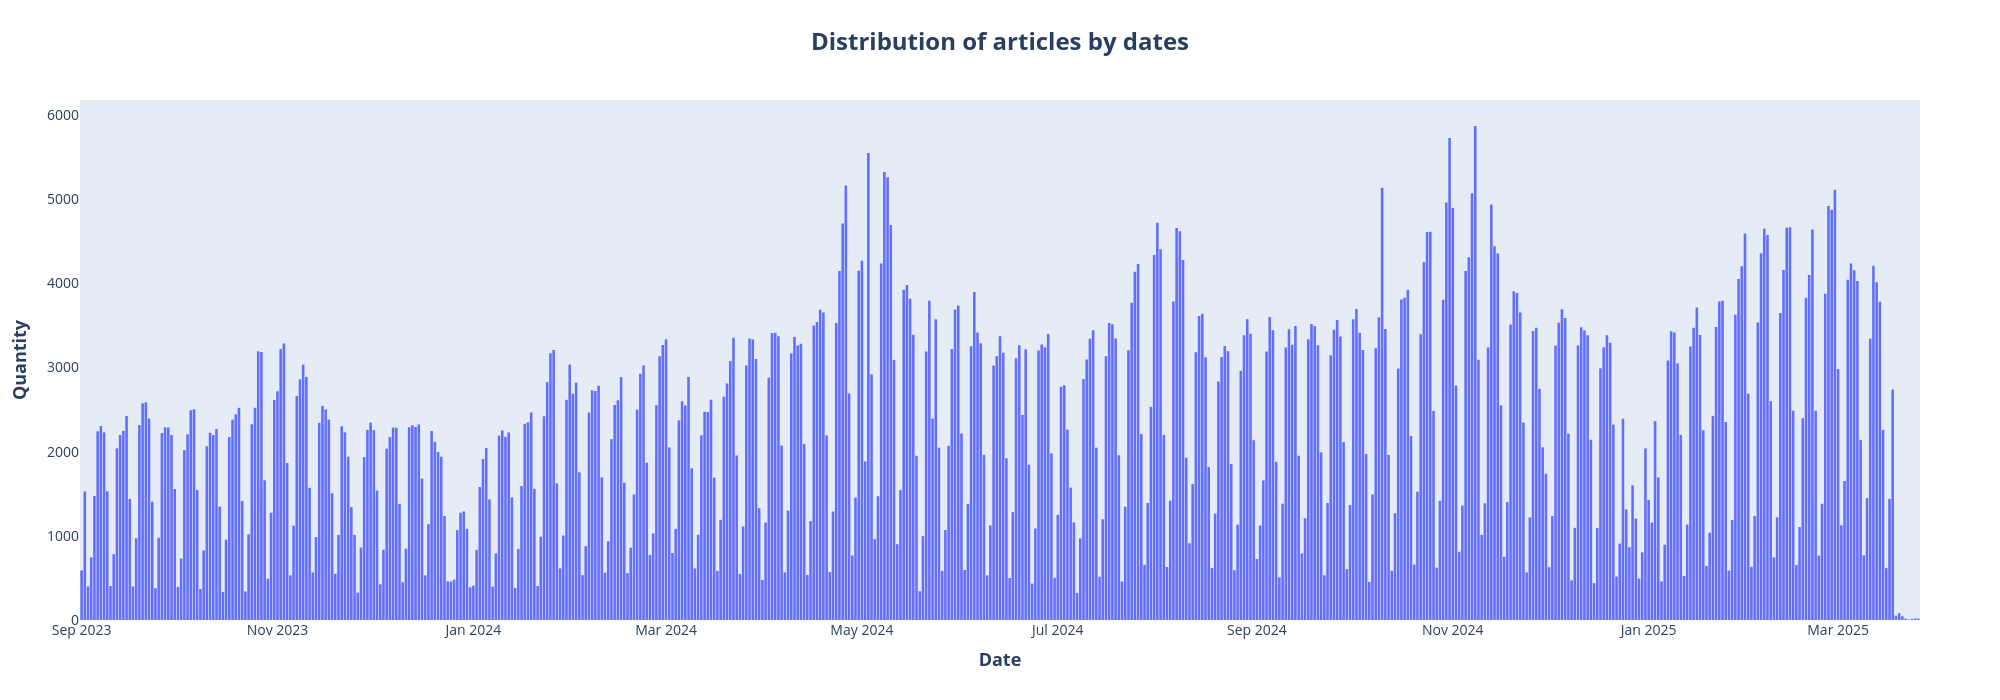
\includegraphics[width=1\linewidth]{img/articles_dist_by_dates.png}
    \caption{Распределение содержащихся в корпусе публикаций по датам.}
    \label{fig:dist_by_dates}
\end{figure}

\textbf{Распределение публикаций по датам.} На Рис. \ref{fig:dist_by_dates} видно, что количество публикаций
колеблется по дням с определённой периодичностью. Детальное изучение показало, что минимумы приходятся
на воскресные и праздничные дни, когда публикуется меньше финансовых новостей. Это естественно отражает
специфику рынка: в выходные и праздничные дни деловая активность снижается, поэтому и публикаций становится меньше.

\begin{figure}[H]
    \centering
    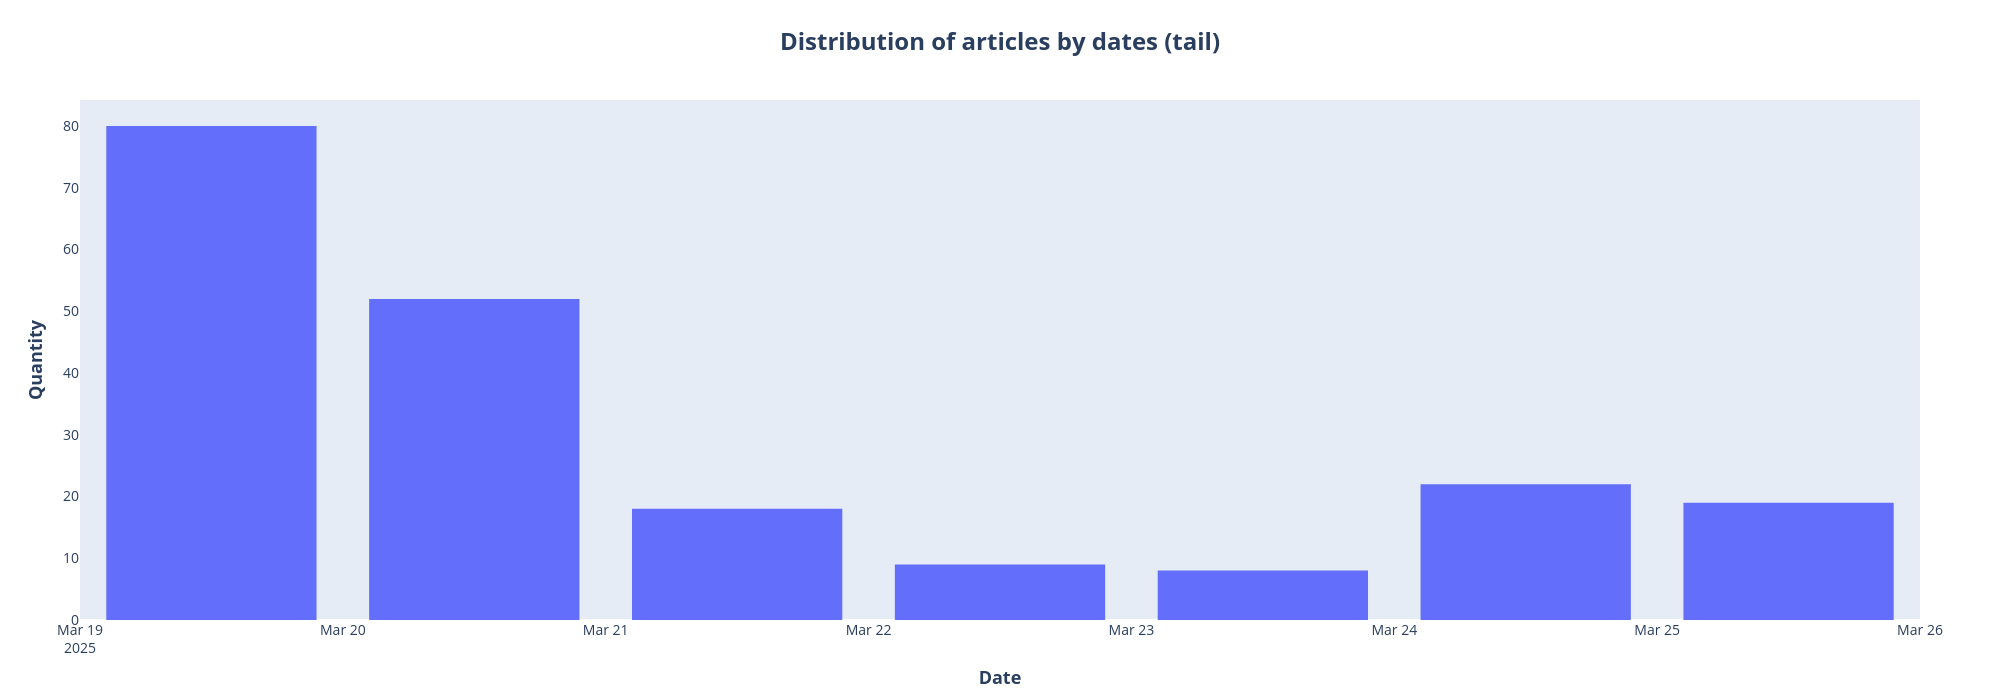
\includegraphics[width=1\linewidth]{img/articles_dist_by_dates_tail.png}
    \caption{\label{fig:dist_by_dates_tail}Распределение содержащихся в корпусе публикаций по датам (хвост).}
\end{figure}

При этом часть статей, по формальным признакам, выходит за границы периода сбора (1 сентября 2023 года --- 18 марта 2025 года).
На Рисунок \ref{fig:dist_by_dates_tail} показаны эти «хвостовые» публикации, численность которых слегка превышает 200 единиц.
Более детальный анализ установил, что публикации фактически были сделаны в установленный интервал, однако их содержание
редактировали или дополняли позже. В результате дата и время публикации на соответствующем сайте обновились, а старая версия
(со старой датой) утрачена. Если бы ссылки парсились не через неделю, а спустя несколько недель и более, таких случаев было
бы несколько больше.


С точки зрения краткосрочного прогнозирования рынка это обстоятельство может привести к искажению временных меток:
часть статей будто бы опубликована позже, чем на самом деле. Поэтому датасет может оказаться менее эффективен
в краткосрочных исследованиях, чем в средне- и долгосрочных (где сдвиг в пару дней уже не так принципиален).
Тем не менее, для данной работы это не играет критической роли, поскольку модель всё равно опирается лишь
на текст статьи и не учитывает точные временные метки публикаций.

\begin{figure}[H]
    \centering
    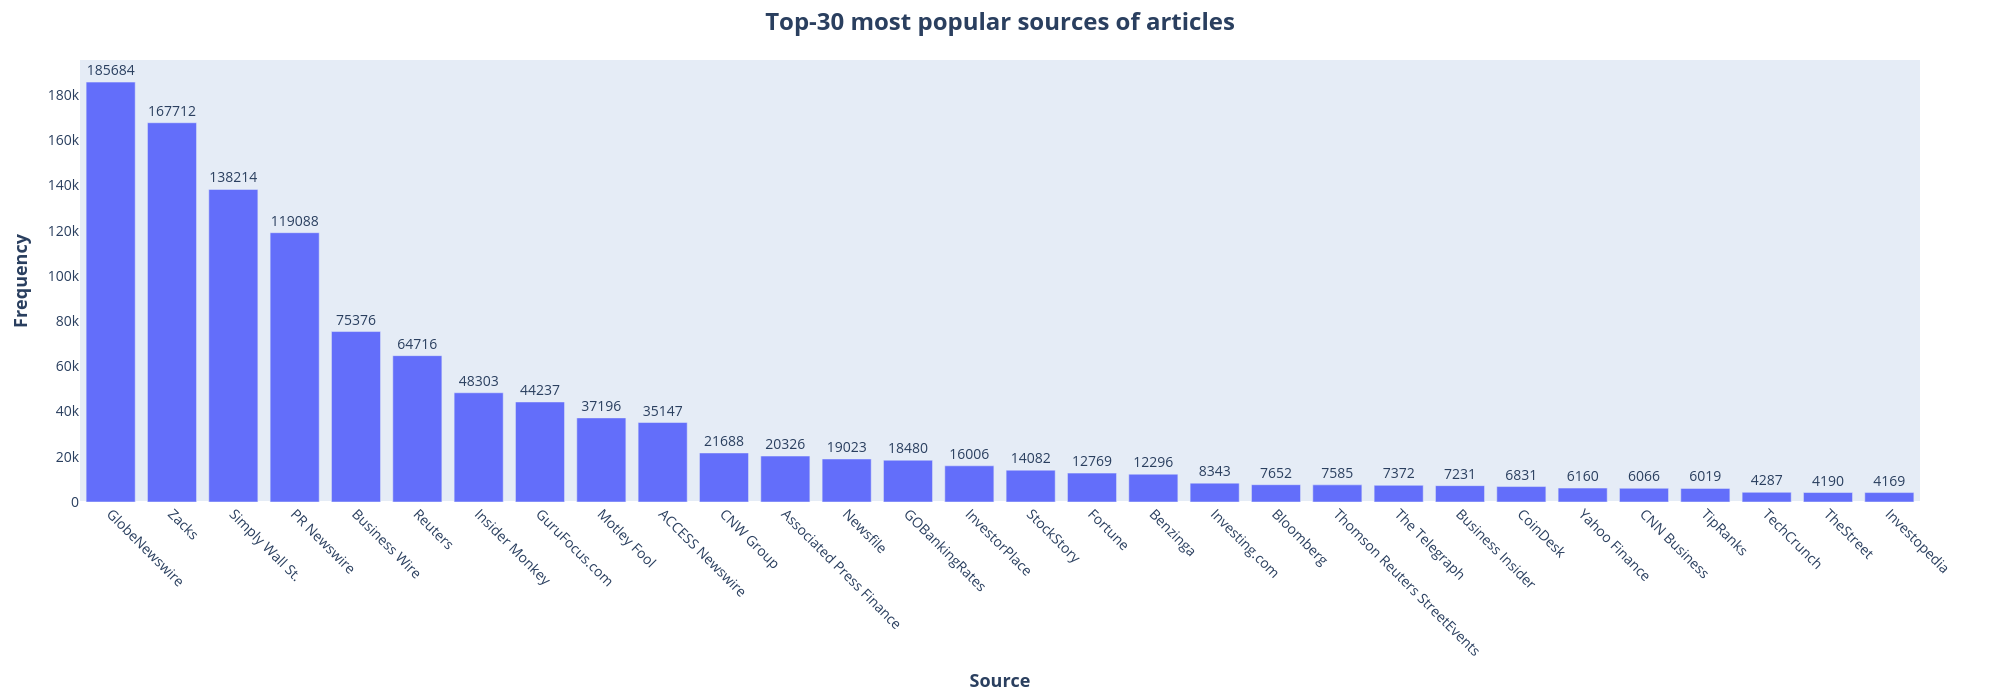
\includegraphics[width=1\linewidth]{img/top30_sources.png}
    \caption{\label{fig:dist_sources}30 наиболее популярных источников финансовых публикаций в корпусе.}
\end{figure}

\textbf{Новостные источники.} Рисунок \ref{fig:dist_sources} иллюстрирует распределение публикаций по 30 наиболее частым источникам.
Анализ показал, что преобладающая доля статей (потенциально 69.2\%) была опубликована полу-автоматизированными агрегаторами:
GlobeNewswire, Zacks, Simply Wall St., PR Newswire, Business Wire, GuruFocus.com, Motley Fool и др. Они фокусируются
на автоматическом сборе ключевых данных с различных ресурсов (регуляторы, официальные сайты компаний и т.п.), публикуя
пресс-релизы, краткие обзоры отчётов и приглашения на корпоративные мероприятия.

В топ-15 источников лишь некоторые можно условно считать «традиционными» новостными ресурсами, такими как Reuters,
Insider Monkey, CNW Group, Associated Press Finance, InvestorPlace. При этом за пределами топ-30 превалируют именно
классические издания, которые в основном публикуют авторские статьи. В реальности же размытая грань между авторскими
и полу-автоматическими материалами усложняет попытки чёткого разграничения.

По приблизительной оценке, из 1 300 000 статей около 900 000 (69.2\%) являются полу-автоматическими.
Это важный фактор для обучения языковой модели, поскольку:

\begin{enumerate}
    \item Качество таких материалов нередко ниже: тексты содержат артефакты, ломаются разметки и вставляются некорректные символы.
    \item Их объём велик, что, с одной стороны, даёт большую семплирующую способность, но с другой — затрудняет очистку и нормализацию без потери значимой информации.
\end{enumerate}

Тем не менее, даже «нечистые» тексты из агрегаторов несут полезную информацию о финансовом рынке и компаниях. Однако, крайне важно разработать корректные правила
очистки и предобработки (см. \hyperref[sec:data_prep]{Раздел 2.2.4}) текстов, чтобы не повредить их семантическую целостность.

Кроме того, и, что более важно, эти полу-автоматические тексты составляют примерно такое же общее количество токенов,
как и «авторские» статьи (30.8\%), несмотря на их количественное доминирование. Следовательно, при правильной обработке
данная группа полу-автоматических статей может дать значимый вклад в обучение языковой модели, не размывая значимость
«авторских» текстов.

\begin{figure}[H]
    \centering
    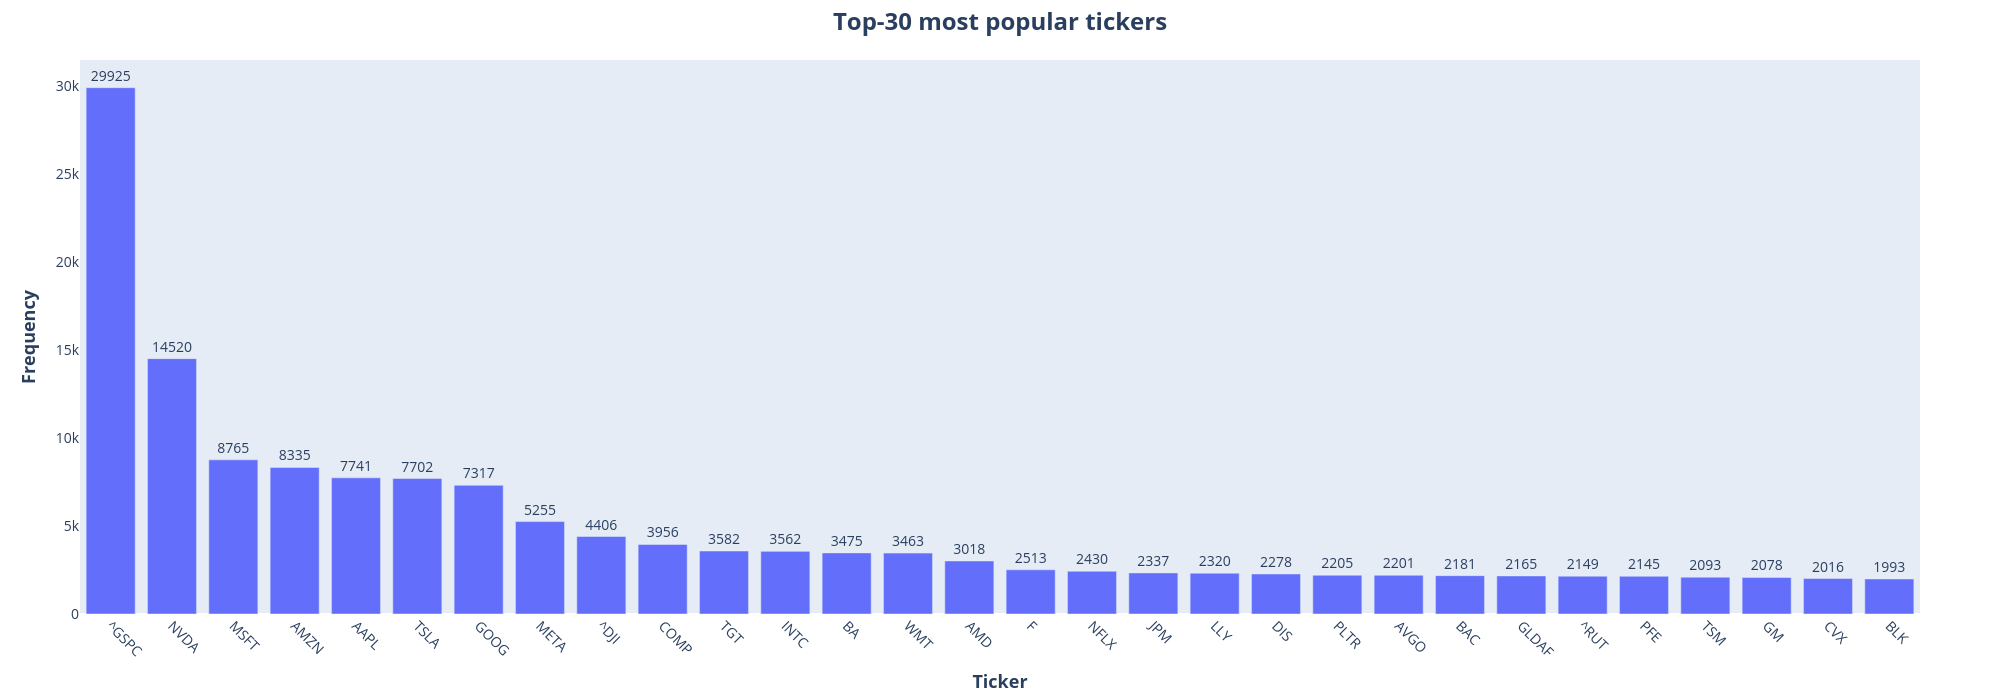
\includegraphics[width=1\linewidth]{img/top30_tickers.png}
    \caption{\label{fig:dist_tickers}30 наиболее частых тикеров в датасете.}
\end{figure}

\textbf{Анализ тикеров.} На Рисунке \ref{fig:dist_tickers} представлено распределение публикаций по 30 наиболее часто встречающимся
тикерам. Лидером является индекс S\&P 500, однако в выборку также попали Dow Jones и Russell 2000. Примечательно, что в топ-10
оказались главным образом IT-компании, причём с существенным отрывом лидирует Nvidia.

При этом около 574 000 (44,2\%) публикаций не содержат вообще никаких тикеров в описании статьи, которое находится
в шапке страницы. Более того, даже когда тикеры присутствуют, они могут отображать не все фактически упомянутые
в статье компании или индексы. Это говорит о том, что данный столбец в датасете, пусть и достаточно репрезентативен,
но не даёт полного покрытия всех потенциальных тикеров, и часть новостей формально «выпадает» из рассмотрения.
Следовательно, для задач, выходящих за рамки данной исследовательской работы стоит создать словарь терминов и наименований,
относящихся к каждому конкретному тикеру, а затем алгоритмически дополнить столбец с тикерами, используя соответствующие тексты.

\begin{figure}[H]
    \centering
    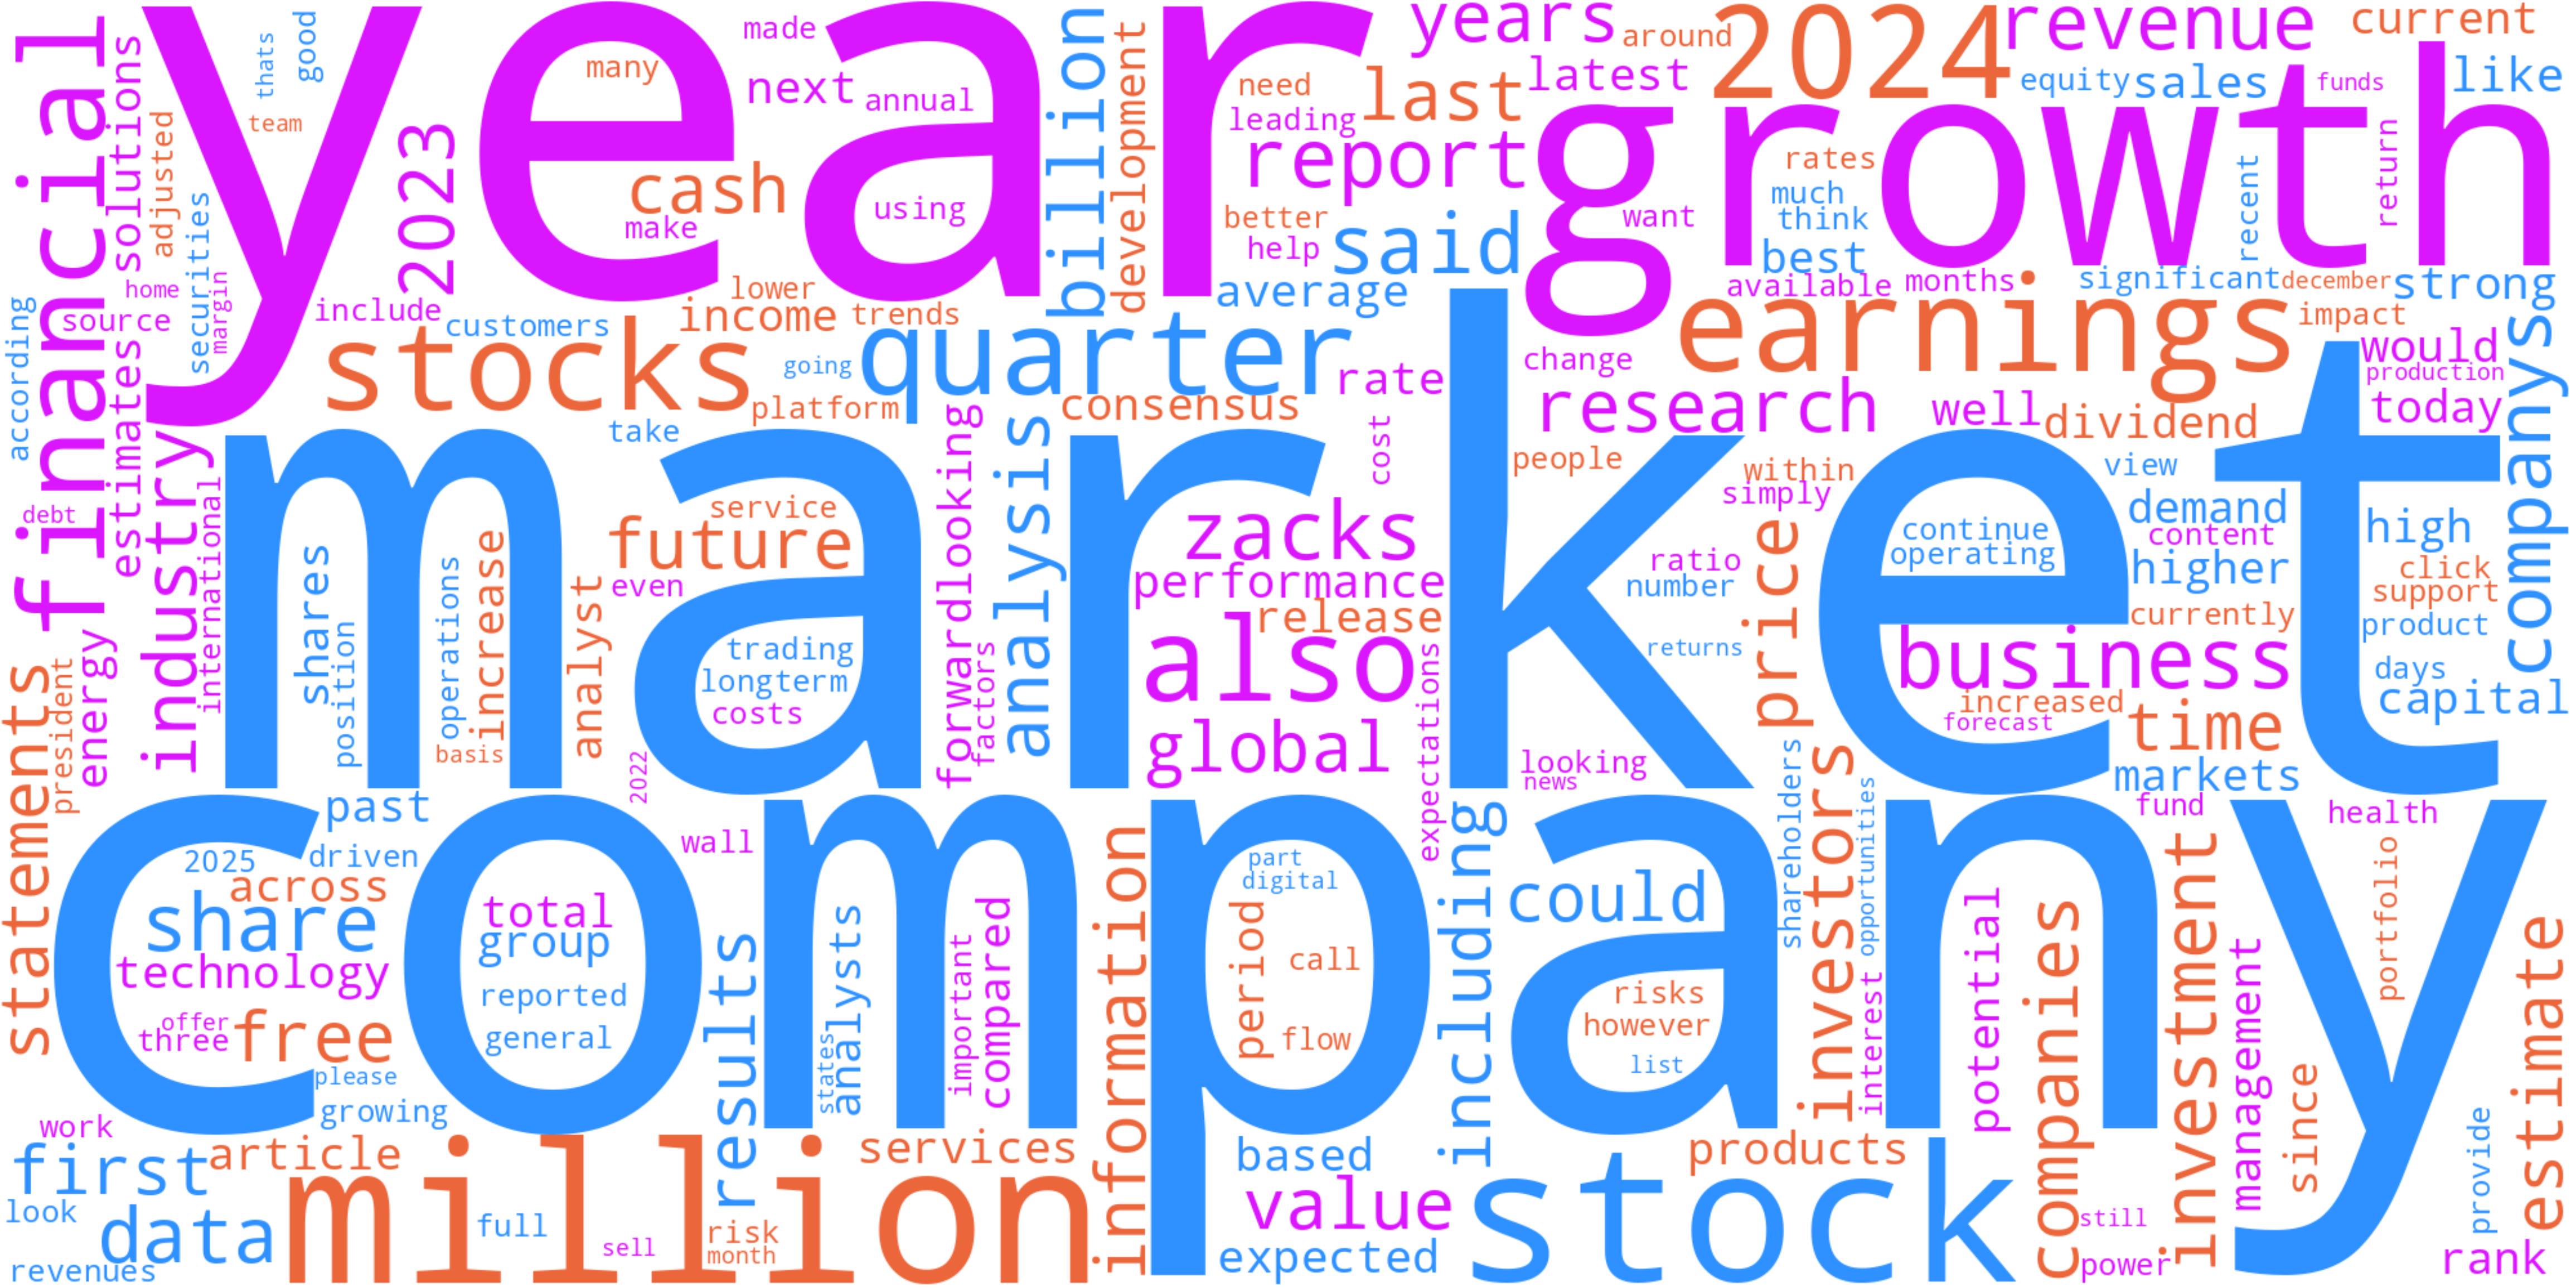
\includegraphics[width=1\linewidth]{img/wordcloud.png}
    \caption{\label{fig:wordcloud}Облако слов, составленное по всем текстам, содержащимся в собранном корпусе.}
\end{figure}

\textbf{Качество текста.} На Рисунке \ref{fig:wordcloud} представлено облако слов, построенное по всему
корпусу собранных текстов. Из этой визуализации можно сделать следующие ключевые выводы:

\begin{enumerate}
    \item \textbf{Репрезентативность данных}. Облако демонстрирует широкий спектр финансовых терминов, что указывает на достаточную репрезентативность
    датасета в финансовой тематике. Это свидетельствует о том, что материал охватывает разнообразные аспекты рыночной деятельности и экономических событий.
    \item \textbf{Специфичность финансовой терминологии}. Распределение частот финансовых терминов существенно отличается от того,
    что наблюдается в популярных корпусах для обучения языковых моделей (например, English Wikipedia или BookCorpus).
    Это различие обуславливает необходимость проведения доменной адаптации DAPT для корректного обучения модели на специфических данных
    финансовой тематики.
    \item \textbf{Уровень шума и наличие нерелевантной информации}. Облако слов включает такие элементы, как «Zacks», «click»,
    «please», «free» и «source». Это указывает на значительное присутствие шумовых, рекламных или автоматически сгенерированных
    фрагментов, что требует разработки специальных методов очистки данных без нарушения семантической целостности текстов.
\end{enumerate}

Дополнительно можно отметить, что выявленные шум и рассеянность терминов могут негативно сказаться на качестве downstream-задач, таких как классификация
или извлечение эмбеддингов, если данные не будут корректно обработаны на этапе предобработки.

\textbf{Вывод}. Собранный датасет новостей характеризуется некоторыми особенностями. Во-первых, наблюдается ярко выраженная сезонность
публикаций --- минимумы приходятся на выходные и праздничные дни, также зафиксированы так называемые «хвостовые» статьи. Во-вторых,
анализ источников показывает, что около 69\% текстов поступают от полу-автоматизированных агрегаторов, что может усложнить процесс очистки
данных, поскольку такие источники нередко порождают тексты с нарушенной разметкой, встроенными артефактами и нерелевантной информацией.
Наконец, выяснено, что датасет обладает высокой вариативностью финансовой терминологии, но в то же время содержит значительный уровень шума,
что в совокупности подтверждает необходимость проведения доменной адаптации (DAPT) и разработки методов для эффективной очистки текстов.

С одной стороны, выявленные особенности (временные сдвиги, шум, доминирование полу-автоматизированных источников) могут
снижать пригодность датасета для краткосрочного прогнозирования или задач, требующих строгой временной разметки. С другой
стороны, для задач, ориентированных на семантическое содержание текста, данные проблемы не оказывают критического влияния.
Надлежащая предобработка, включающая очистку текстов и устранение нерелевантных элементов, позволит существенно повысить качество
обучаемой модели и расширить ее возможности для обобщения на различные типы публикаций.

\subsubsection{Предобработка данных}
\label{sec:data_prep}
После проведения локального и глобального анализов текстовых данных, в ходе которых были выявлены как шумовые
паттерны внутри отдельных документов, так и системные аномалии, свидетельствующие о нерепрезентативности некоторых
публикаций в корпусе в целом, был спроектирован многоэтапный потоковый пайплайн предобработки на лету с использованием
чанков по 100 000 публикаций. Ключевым ограничением при разработке решения стала ограниченность оперативной памяти: при
объёме исходного корпуса порядка 15 ГБ стандартные операции фильтрации и полного прохода по текстам требовали выделения
значительного константного буфера памяти. Это породило необходимость адаптации алгоритма к потоковой обработке порциями
фиксированного размера.

В ходе первого этапа каждый чанк загружался из хранилища и сразу подвергался первичной фильтрации: документы,
содержащие менее 100 символов, отбраковывались как недостаточно информативные. Эмпирически установленный порог
в 100 символов оказался достаточен для устранения «пустых» артефактов, возникающих из-за нестабильности разметки
на стороне источников. Так, на популярных площадках вроде Yahoo! Finance текст порой оказываются зашитым внутри
нетипичных HTML-тегов — например, в ‘<tbody>’ вместо привычного ‘<p>’ — что приводит к появлению почти полностью
пробельных записей или маркетинговых вставок в конце документа.

Следующим шагом реализован фильтр по заголовку: на его основе формализованы 66 правил, охватывающих как общие
шаблоны («Form 8», «Net Asset Value», «Holdings in company»), так и более таргетированные для шумных 12 источников
(например, в GlobeNewswire удалялись заголовки, содержащие «Declaration» или начинающиеся с «Key digital»). Такая
селекция гарантировала удаление публикаций, состоящих преимущественно из табличных данных или кратких заполнителей.

После нормализации всех видов пробельных символов — слияния подряд идущих пробелов или переносов строк в единичный
символ, замены неразрывных пробелов ‘\\xa0’ на стандартный пробел и унификации специальных знаков в тексте ---
применялись ещё 12 правил, направленных на отбраковку нерепрезентативных документов по содержанию основного тела
публикации. В частности, всё, что начиналось с маркера «(Repeat)», а также приветственные шаблоны специфичных
источников вроде «Dear madam, sir, please find hereunder the links» для GlobeNewswire, автоматически исключалось
из дальнейшей обработки.

Далее текст очищался от контактных данных и типовых футеров: ссылки, адреса электронной почты, а также фразы,
однозначно указывающие на конец документа («Forward-looking statements», «Contact Details»), либо нерепрезентативность
абзаца («Source:», «See More:», «Sponsored:»). Кроме того, из начала публикаций удалялись стандартные вводные фразы вроде
«The recommendations of Wall Street analysts» и «When deciding whether to buy, sell, or hold a stock, investors often
rely on analyst recommendations». Всего в различных группах было сформировано 92 правила очистки.

Такое агрессивное очищение текстов обуславливается тем, что отфильтрованные паттерны встречаются настолько часто,
что крайне негативно сказываются на кластеризации искусственно завышая метрику кластеризации. После проведенном
агрессивном очищении корпуса, метрика качества действительно уменьшилась, однако кластеры стали гораздо более
репрезентативными и основанными на семантике самой новости, а не ее источниках, маркетинговой и правовой информации
в текстах.

\begin{figure}[H]
    \centering
    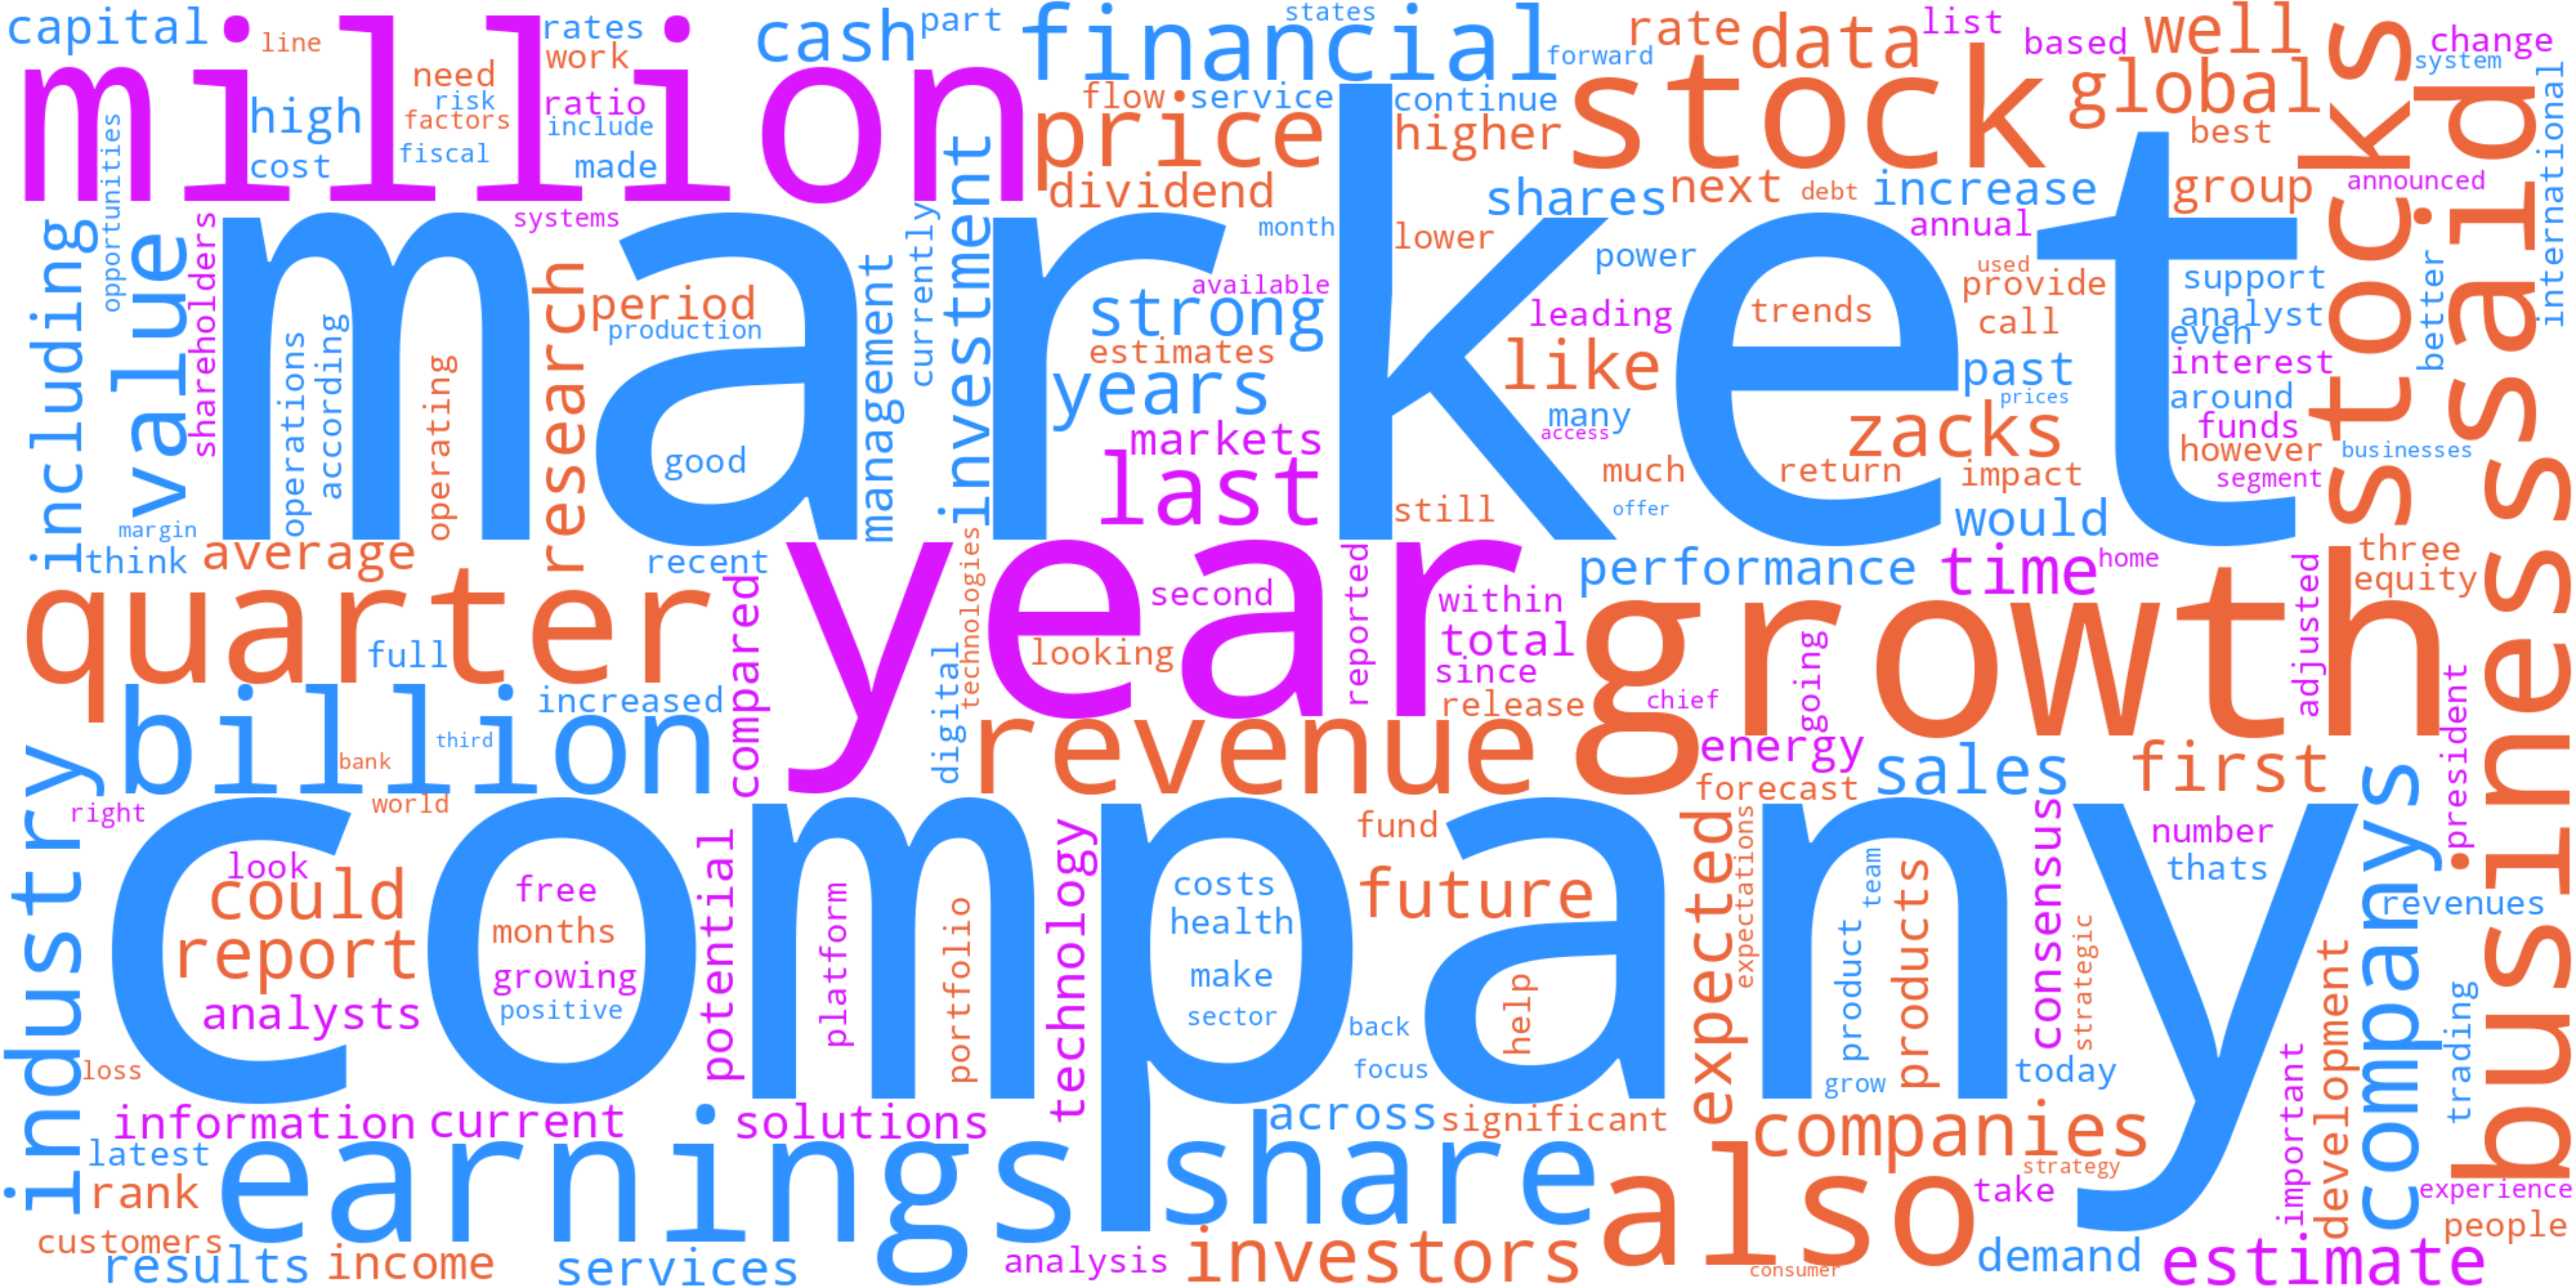
\includegraphics[width=1\linewidth]{img/prep_wordcloud.png}
    \caption{\label{fig:prep_wordcloud} Облако слов, составленное по всем по текстам, содержащимся в предобработанном корпусе.}
\end{figure}

В качестве валидации качества очистки текстов можно обратиться к облаку слов корпуса после предобработки (Изображение \ref{fig:prep_wordcloud}),
на котором отчетливо видно улучшение: отсутствуют такие слова, как 'forwardlooking', 'link', 'click', 'simply' (название источника Simply Wall St.) и другие.

Наконец, перед сохранением чанков происходила сортировка по дате публикации и удаление дубликатов на основе полного текста документа.
С учётом описанных операций объём корпуса сократился с 15,4 ГБ в формате CSV (8,6 ГБ в Parquet) до 5,9 ГБ (2,0 ГБ в Parquet): из 1 304 717
исходных записей осталось 1 267 416, то есть удалено было всего 2,8\% документов. Данный результат свидетельствует о высокой
доле шумов в тексте в собранном датасете и подчёркивает эффективность многоступенчатого потокового подхода к предобработке,
который сохраняет оперативную память и обеспечивает качественную очистку текстовых данных перед последующими этапами
тематического моделирования и анализа.
